
%%% Local Variables: 
%%% mode: latex
%%% TeX-master: "main"
%%% End: 
\section{Initial Assembly}


% This section should highlight the comparison between the full-data assembly and that conducted with only the properly paired reads.
% It should emphasize the larger number of ORFs recapitulated by the properly paired reads, and the improved mappability of such a dataset.
% Therefore, at the cost of lower effective sequencing depth, transcripts from the properly paired dataset are less likely to be false positives resulting from the low mappability of improper pairs.
Initial transcriptome assemblies were conducted for the full dataset and the subset of properly-paired reads. Hypothetically, extra improperly-paired or unpaired reads could have been terminal or bridging reads, which would have increased the precision of boundary estimates. Alternatively, the properly-paired subset could have resulted in a simpler and cleaner graph for traversal by the assembly algorithm. Both of the resulting assemblies were compared by their qualities, such as assembly size, transcript lengths, and inclusion of the reference protein annotations. 

In this comparison, the assemblies were inspected for errors that affect these qualities. The previous chapter described techniques for the minimization of background signals that are frequently ignored and not quantified by similar studies. Automated methods such as assembly can have difficulty when background and overlapping signals are sufficiently complex. Therefore, the results were inspected for misassemblies, artifacts from the graphs constructed for the dataset. Documentation and analysis of these artifacts was required to select the best assembly.

\begin{table}
\caption{Assembly Comparison}\label{table:assemb_compare}
\begin{center}
\begin{tabular}{|c|c|c|}\hline
  & All Reads & Proper Pairs\\\hline\hline
Transcripts & 3054 & 4295\\\hline
Sequenced Mb & 6.1 & 7.2\\\hline
Length Range & 200-28kb & 200-35kb\\\hline
CDSes & 2397 (63\%) & 3225 (85\%)\\\hline
Standard Transcripts & 796 (27\%) & 1029 (24\%)\\\hline
Standard Mb & 3.7 (61\%) & 4.56 (63\%)\\\hline
Novel Transcripts & 2129 (73\%) & 3266 (76\%)\\\hline
Novel Mb & 2.4 (39\%)& 2.64 (37\%)\\\hline
\end{tabular}
\end{center}
\end{table}

\subsubsection{Assembly Comparison}
First, simple statistics were compiled for both assemblies (\ref{table:assemb_compare}). The transcripts that contained reference protein annotations (referred to as ``standard'' transcripts), were only about 25\% by number but accounted for 63\% of the assembled basepairs for both datasets. Upon inspection, the assembly from the subset of properly-paired reads was larger and more inclusive, recalling 85\% of the reference ORFs. Also, this assembly had higher per-base sequencing depth in both ``standard'' and ``novel'' transcripts (\ref{fig:5.1}). While the transcript lengths were comparable (\ref{fig:5.2a}), the assembly from all reads had lower expression, size, and inclusiveness of the reference CDSes compared to the subset. Therefore, the transcript coordinates from the uncurated properly-paired assembly were used for further analysis of feature length, UTR length, and expression.




\begin{figure}
\small
\begin{center}
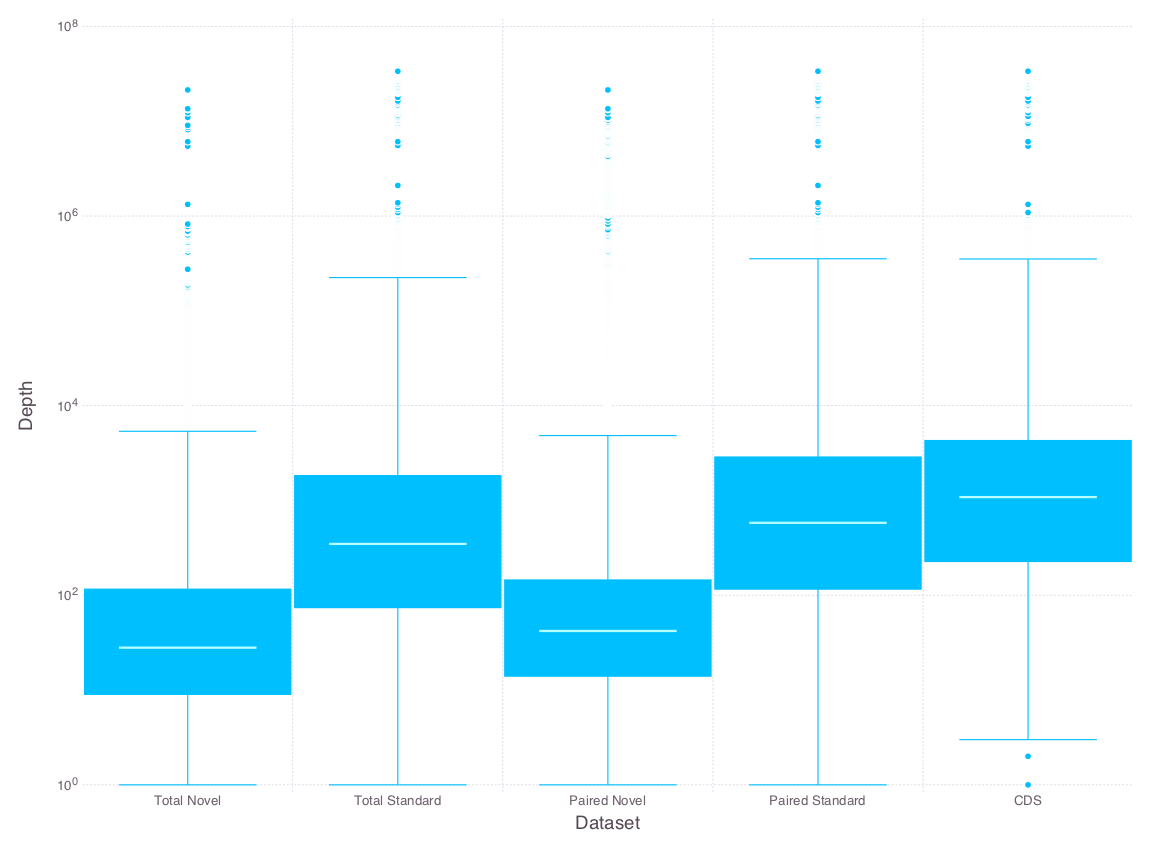
\includegraphics[width=0.8\textwidth,height=3.25in]{images/Assembly/Comparison/PairvsTot_boxplot.png}
\end{center}
\caption{Transcript Depth Comparison}\label{fig:5.1}
\end{figure}


\begin{figure}[t]
\small
\begin{center}
\begin{minipage}{.5\textwidth}
\begin{center}
{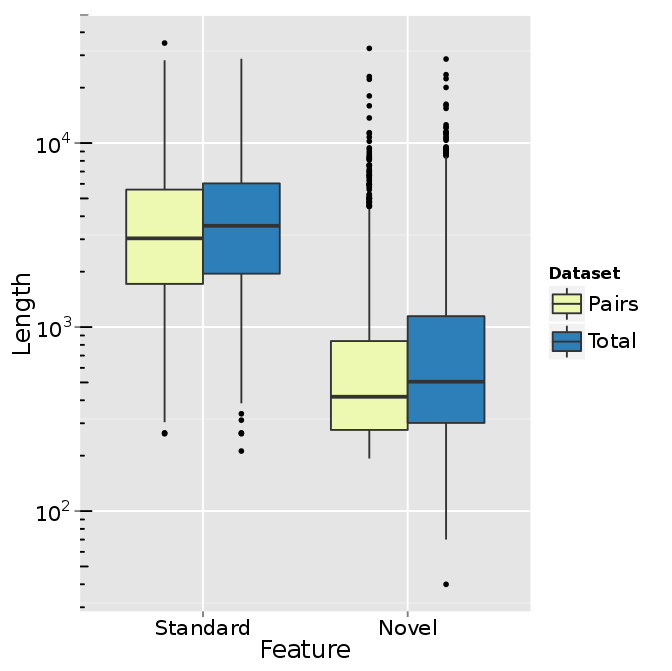
\includegraphics[width=\linewidth,height=2.5in]{images/Assembly/Comparison/TotvsPaired_length.png}
\subcaption{Length Comparison}\label{fig:5.2a}}
\end{center}
\end{minipage}%
\begin{minipage}{.5\textwidth}
\begin{center}
{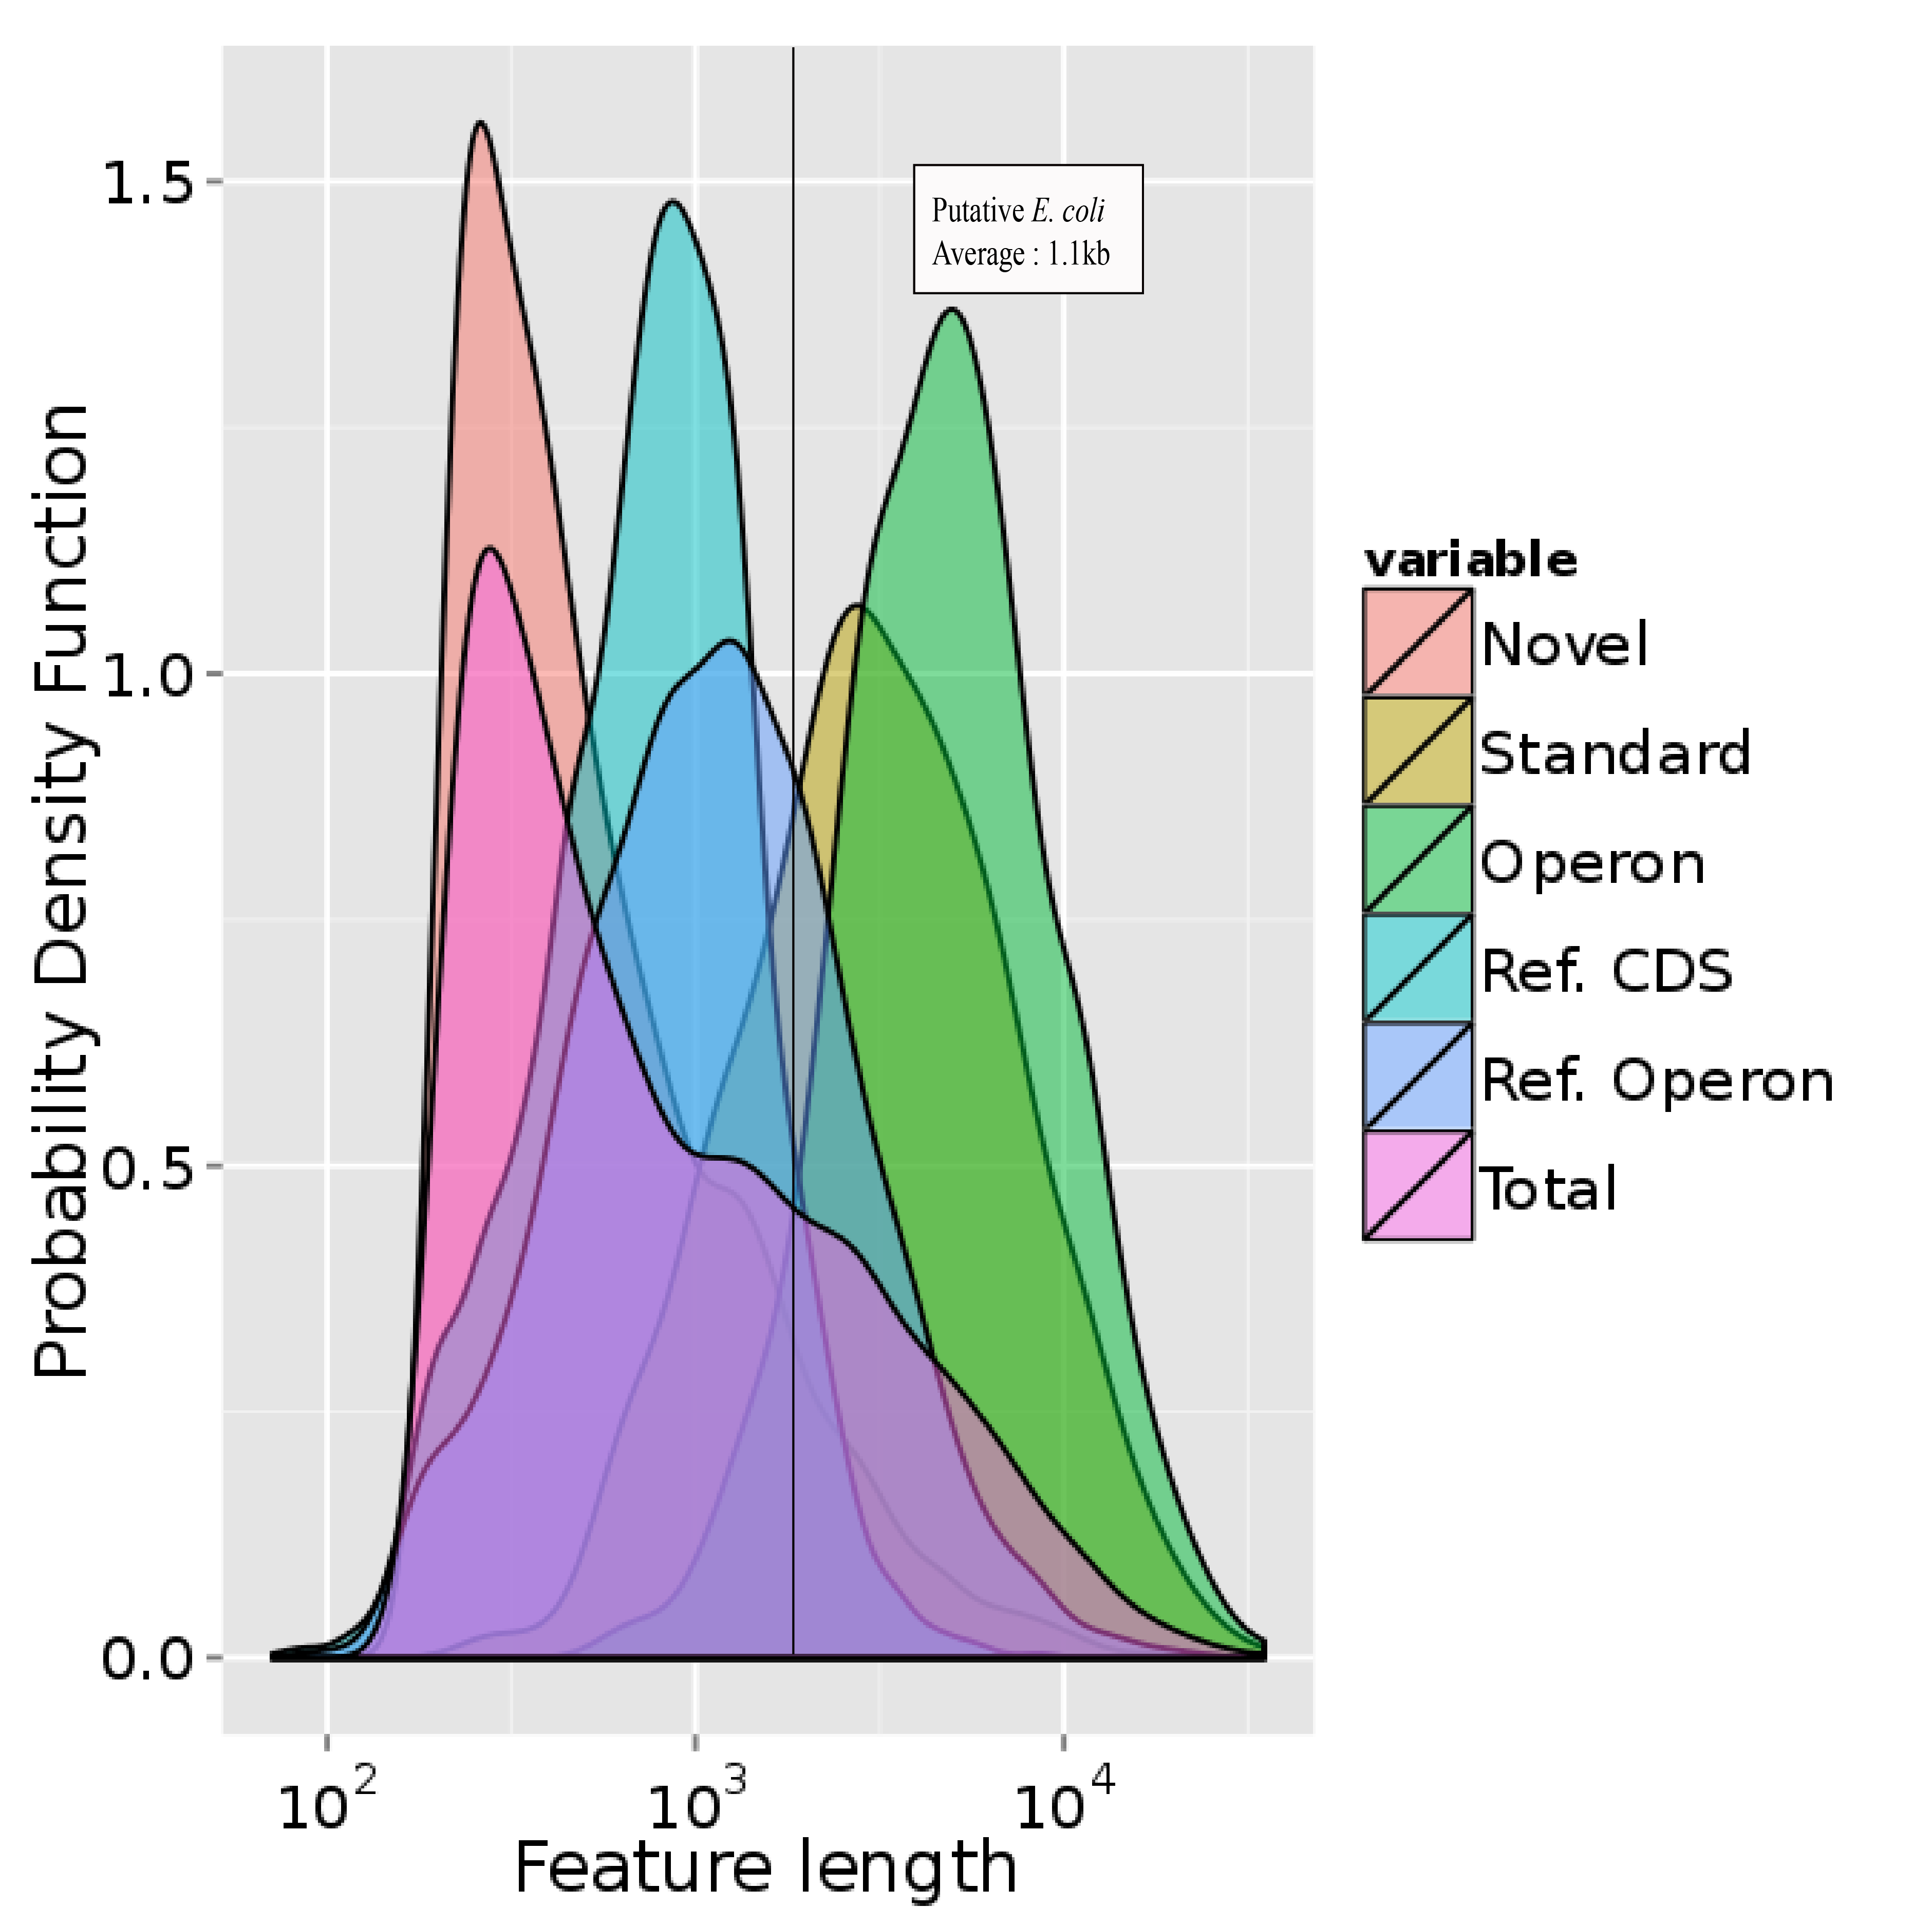
\includegraphics[width=\linewidth,height=2.5in]{images/Assembly/Summary/ffeature_length_1.png}
\subcaption{Feature Lengths}\label{fig:5.2b}}
\end{center}
\end{minipage}
\end{center}
\caption{Transcript Length Comparison and Uncurated Feature Lengths}
With improved inclusiveness (Table \ref{table:assemb_compare}), expression levels(Figure \ref{fig:5.1}), and comparable transcript sizes \subref{fig:5.2a}), the uncurated assembly from the properly-paired reads was selected for further evaluation. \subref{fig:5.2b}) Mono and polycistronic transcripts are present along with 3120 putative novel transcripts. The standard transcripts are close in size to prokaryotic norms\cite{86}.
\end{figure}


\subsubsection{Uncurated Assembly Statistics}

In the uncurated assembly, 4177 transcripts spanning 7.18Mb were assembled. This size is 88\% of the maximum possible size of the transcriptome. Each of these transcripts aligned to a single location in the genome with \textgreater 98\% identity and less than 30bp of gaps, indicating success and quality of the assembly results. Of these, 1029 standard transcripts spanning 4.56Mb contained 3225(86\%) reference protein annotations. The remaining 3120 (75\% by number, 36.5\% by basepairs) were putative novel transcripts, lengths ranging from 200-32.7kb. A large and rich transcriptome was suggested by these whole-transcriptome statisics.

\begin{figure}[h!]
\small
\begin{center}
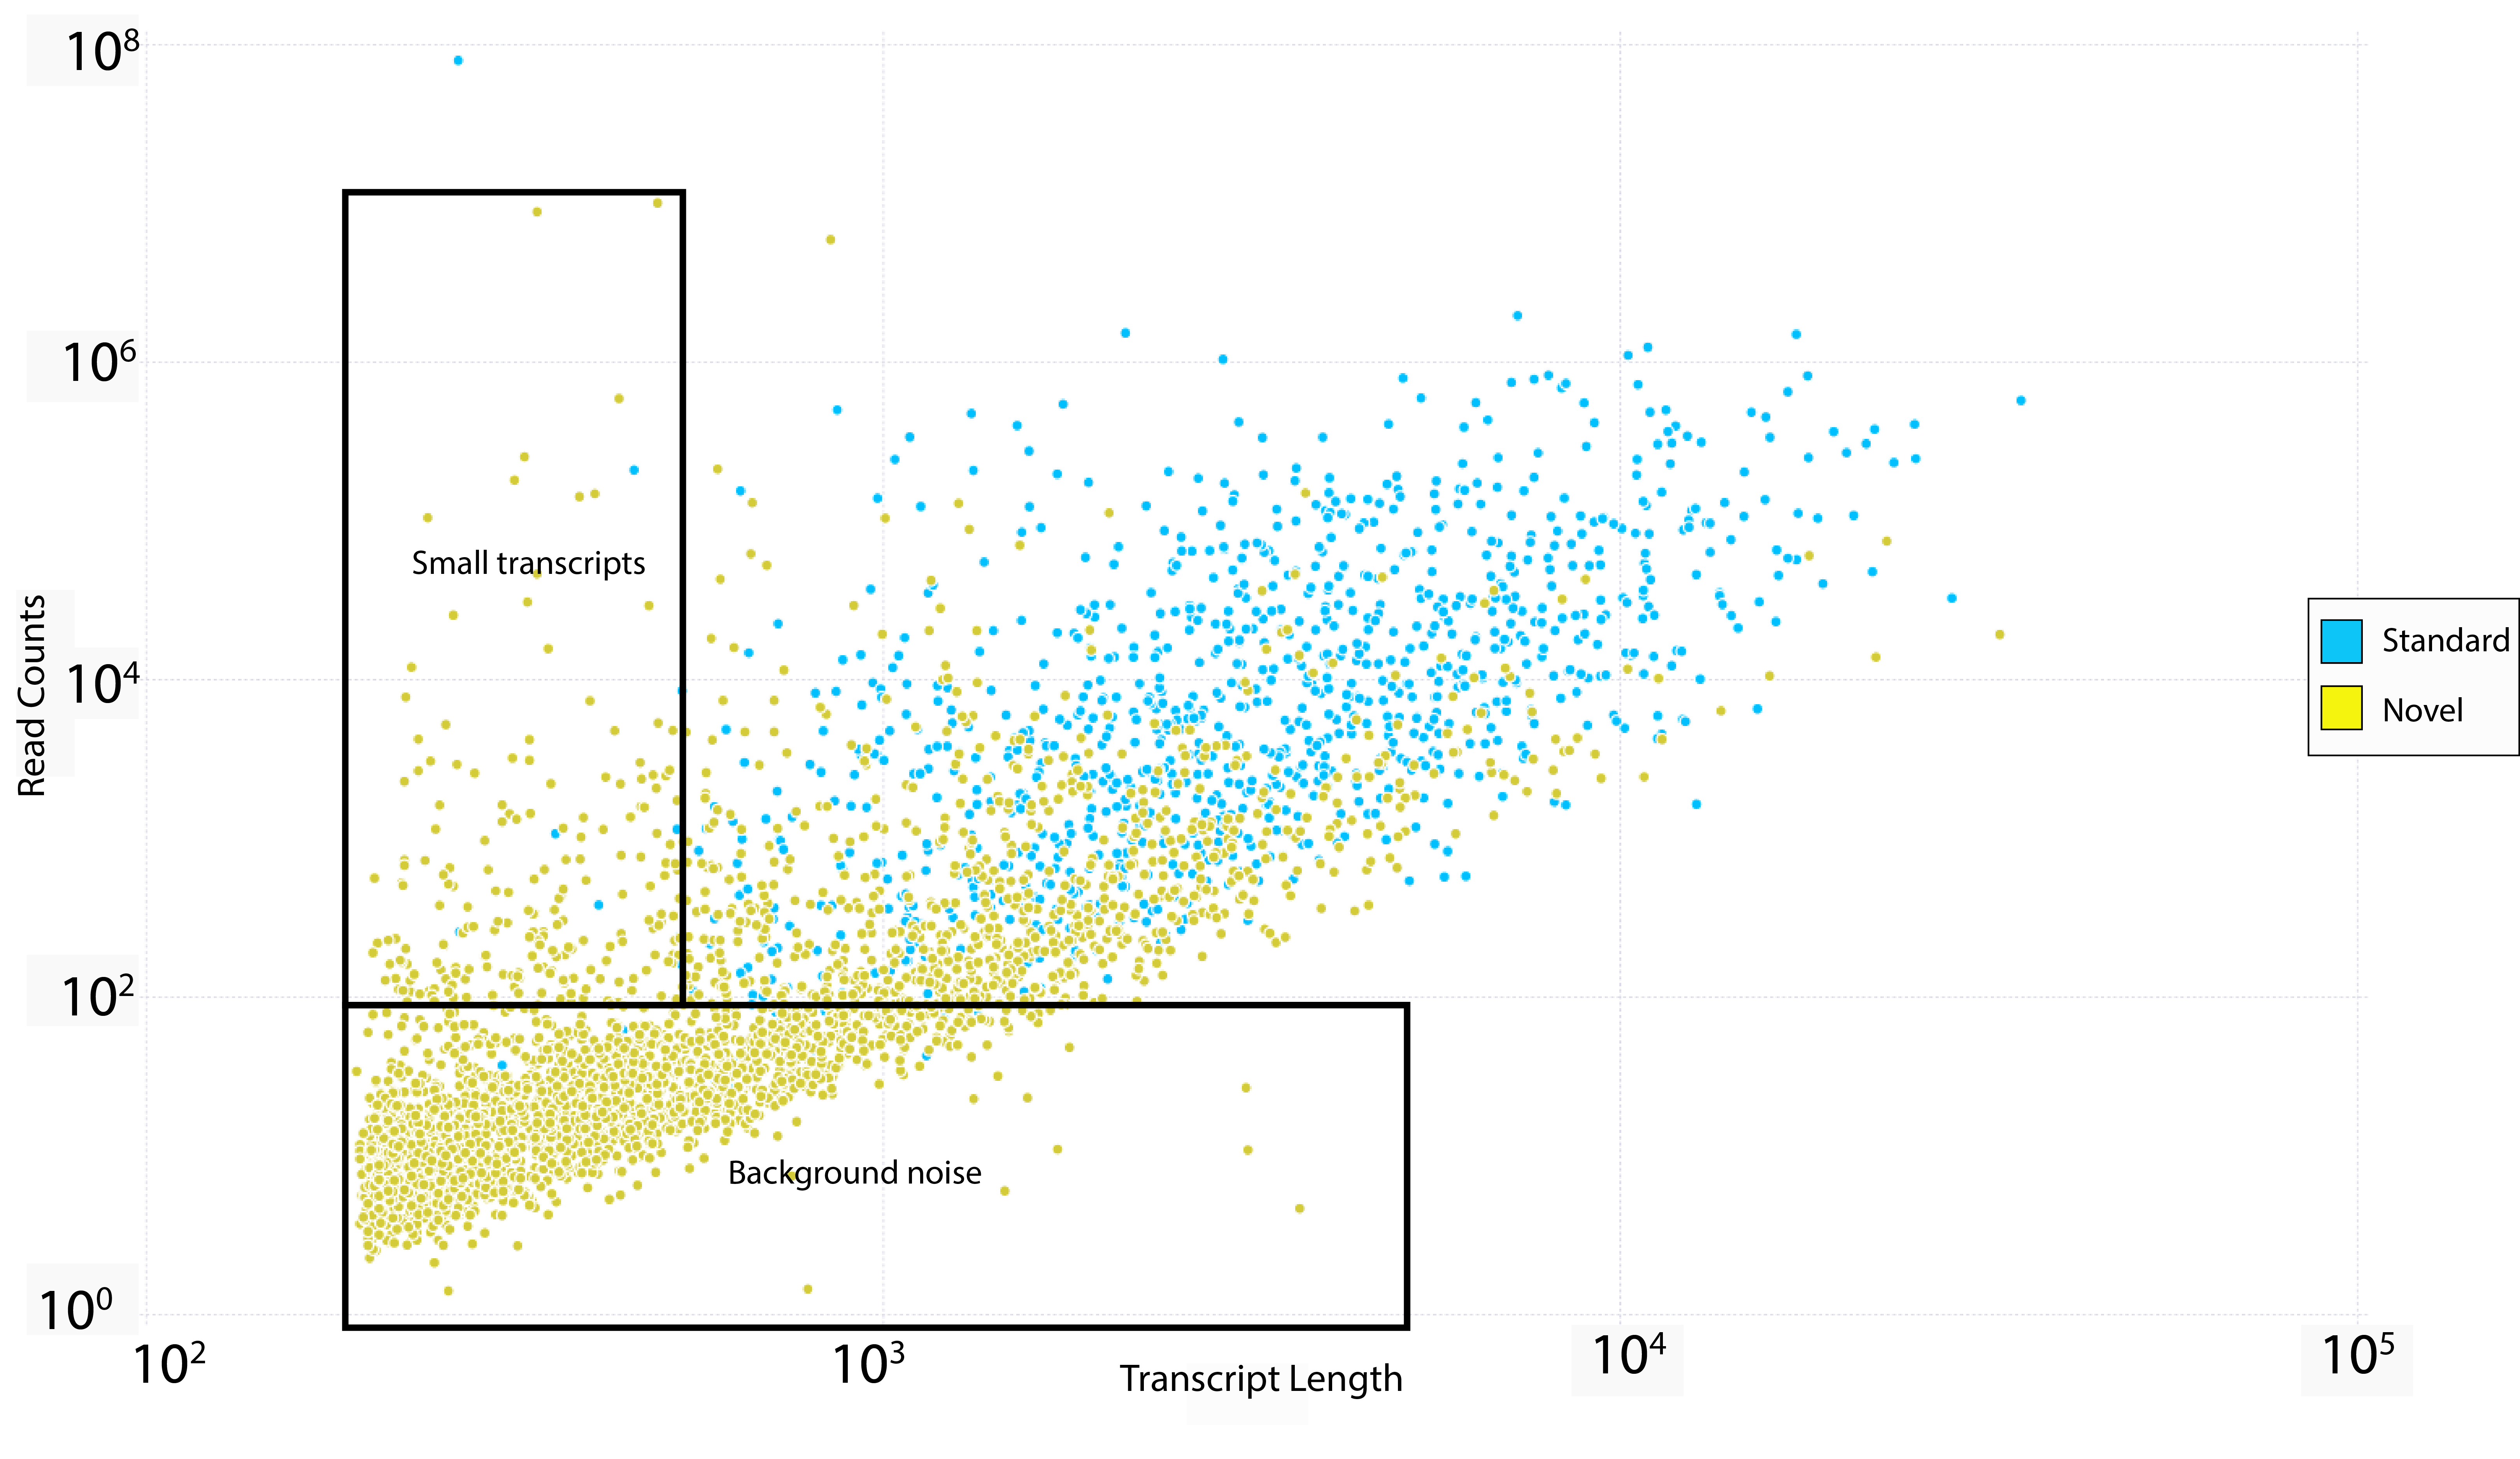
\includegraphics[width=\textwidth,height=4in]{images/Assembly/Summary/Depth_vs_length.png}
\end{center}
\caption{Read Count vs Transcript Length}\label{fig:5.3}
Three additional populations are present in the assembled transcripts. Short novel transcripts with high expression are candidates for \textit{cis}-encoded antisense small RNAs. Those that are long in length with weaker expression tend to be found antisense from a standard transcript and thus represent background antisense signal (\textless 5\% sense expression). However, the majority of the novel transcripts are short in length with weak transcription and most likely represent background signals such as spurious transcription.
\end{figure}

Additional data show the characteristics of the transcripts themselves and paint a more complicated picture. The standard transcripts, including mono and poly-cistronic transcripts, were larger than the novel set(\ref{fig:5.2b}). More surprisingly, they were larger on average than estimates of the mean transcript size in \textit{E. coli}\cite{86}. In addition, the standard set also possessed higher levels of expression(\ref{fig:5.1}). Together, there was a trend between length and expression that divided the novel transcripts into distinct types(\ref{fig:5.3}). The majority of the novel transcripts were short in length (200-500bp) with low read counts. Depending on local depth and annotation patterns, some of these putative transcripts could have been technical artifacts. Longer novel transcripts with similarly low read counts were most likely assemblies of background (1-5\%) or antisense signal. Outside of these troubling groups, there were a number of highly expressed, short, novel transcripts that could have been small peptide encoding transcripts or small RNAs. Equally expressed and larger transcripts could also represent novel transcripts and protein encoding genes. The trend between transcript length and expression indicates the presence of both novel transcripts and technical artifacts in the assembly results, necessitating further investigation and correction.


\begin{figure}
\small
\begin{center}
\begin{minipage}{.5\textwidth}
\begin{center}
{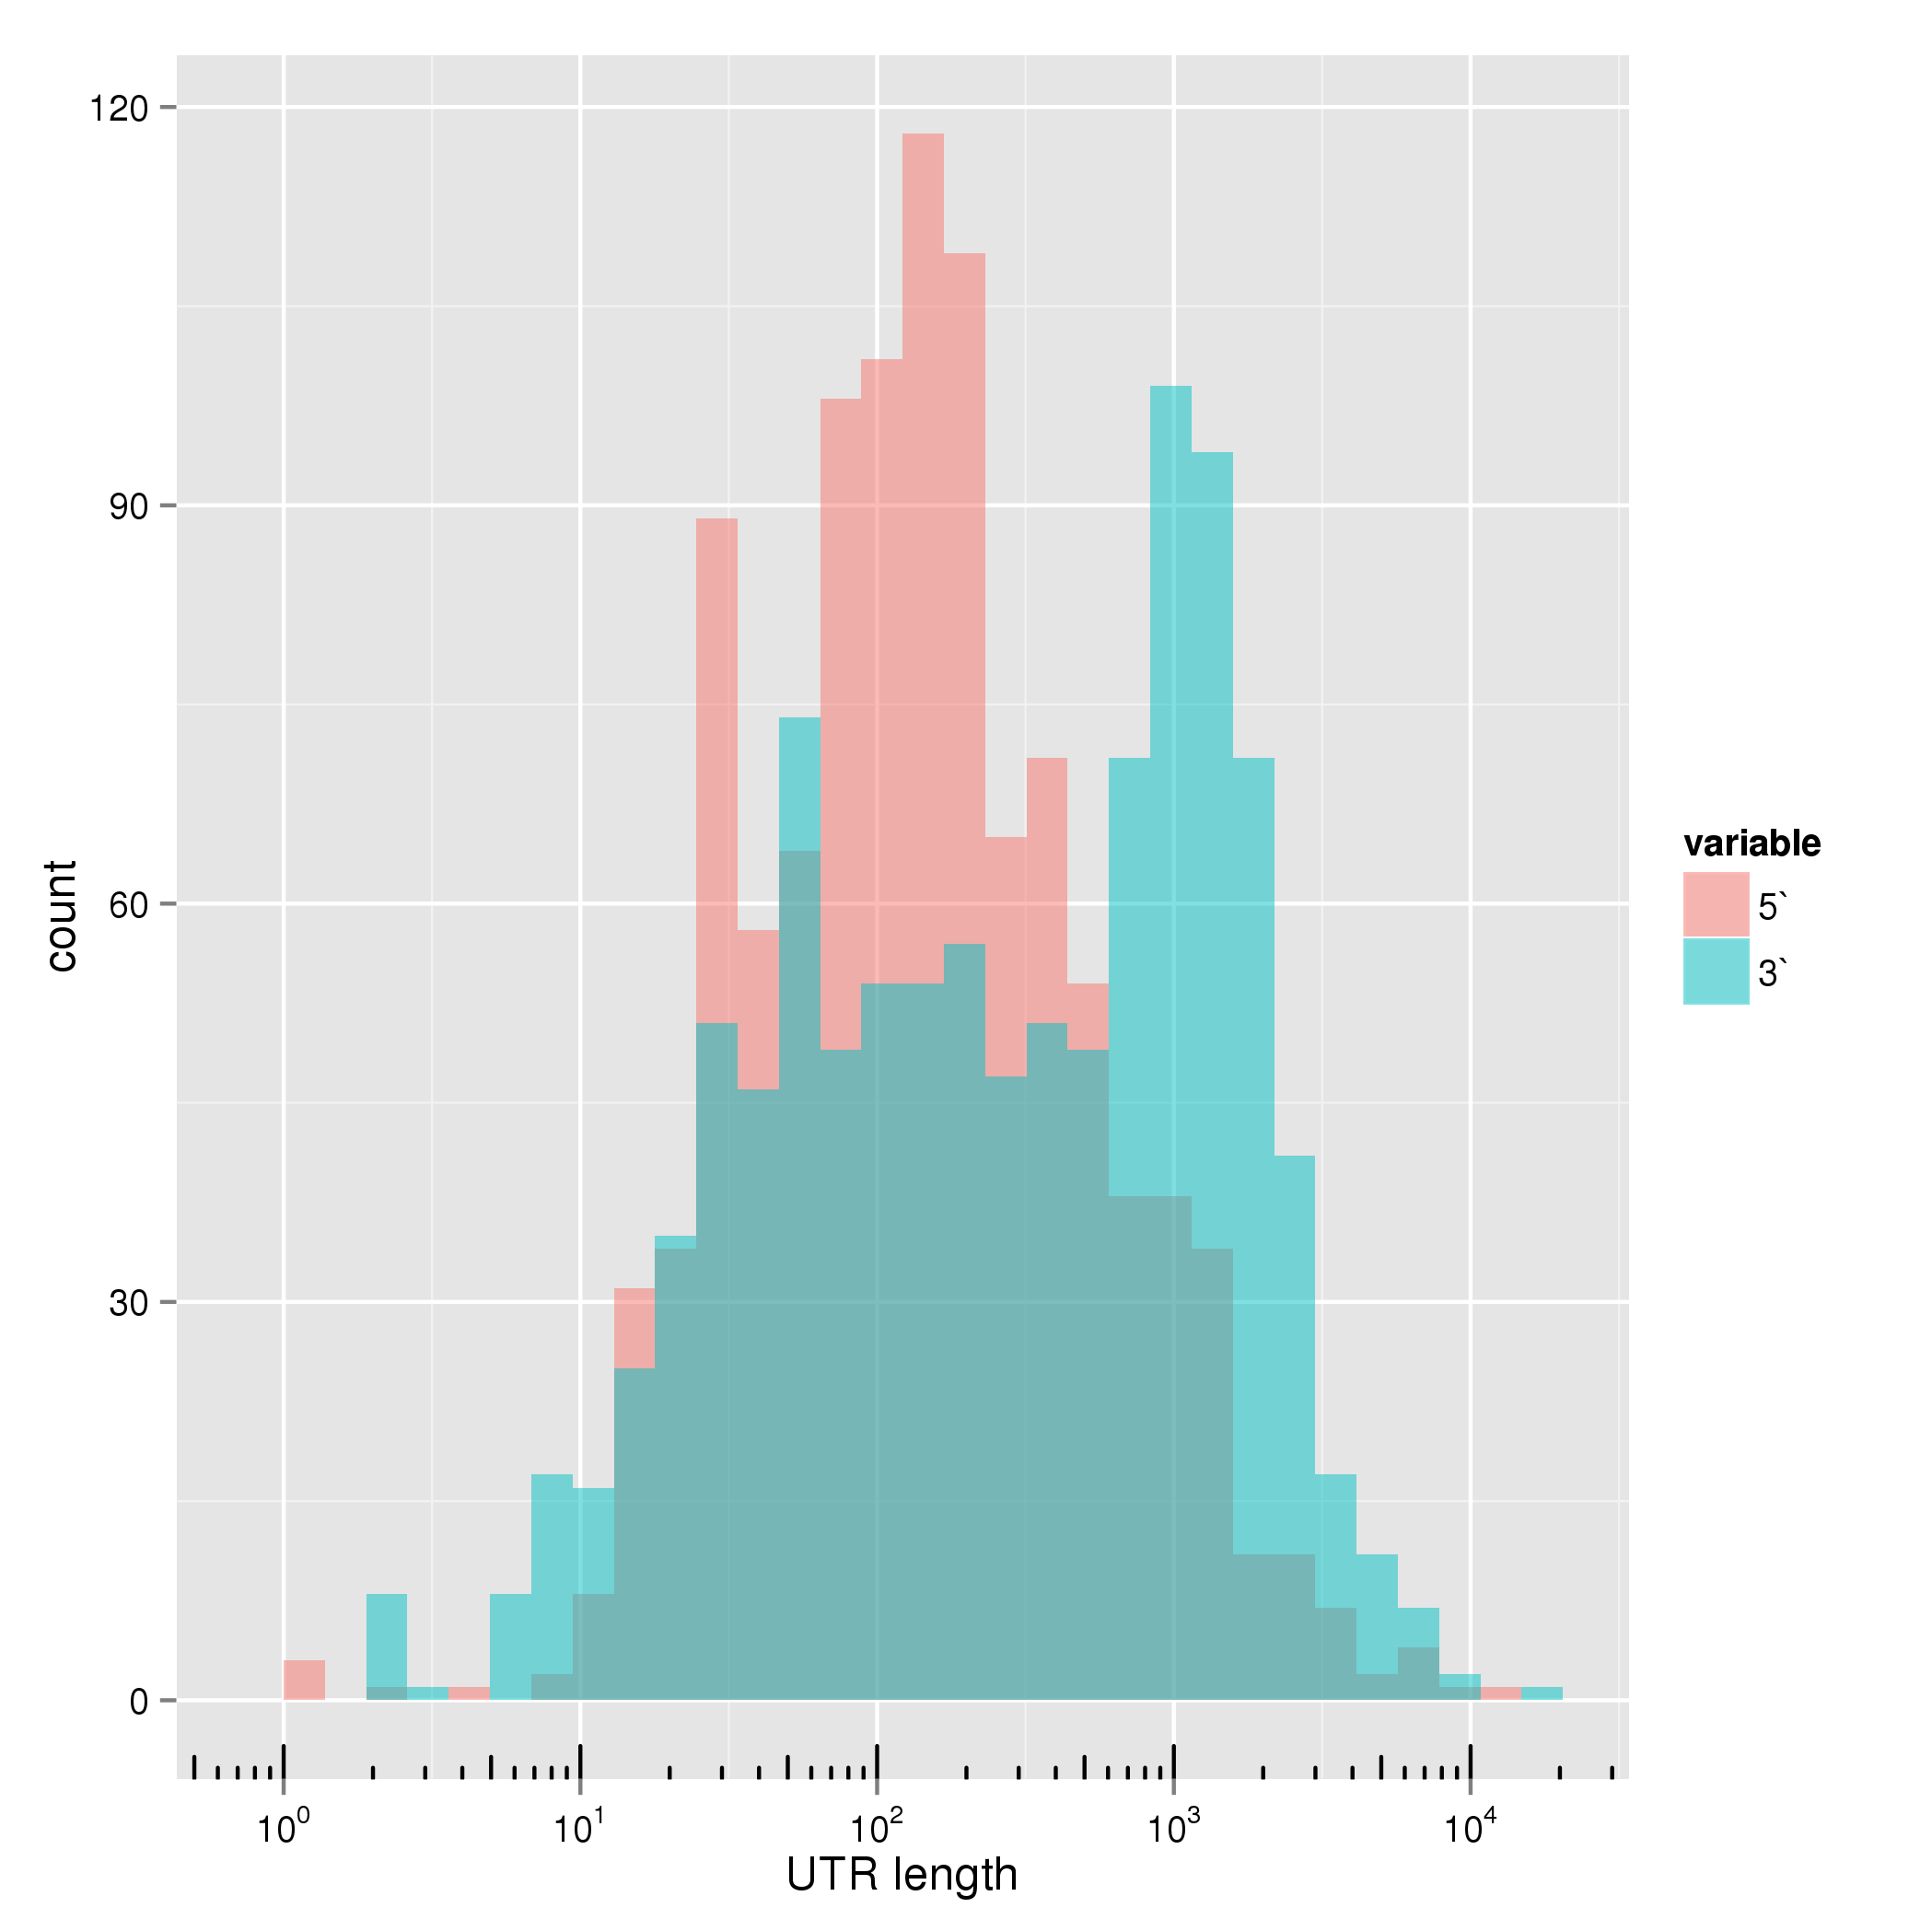
\includegraphics[width=\linewidth,height=3in]{images/Assembly/Summary/futrlength.png}
\subcaption{5$\prime$ and 3$\prime$ Untranslated Regions}\label{fig:5.4a}}
\end{center}
\end{minipage}%
\begin{minipage}{.5\textwidth}
\begin{center}
{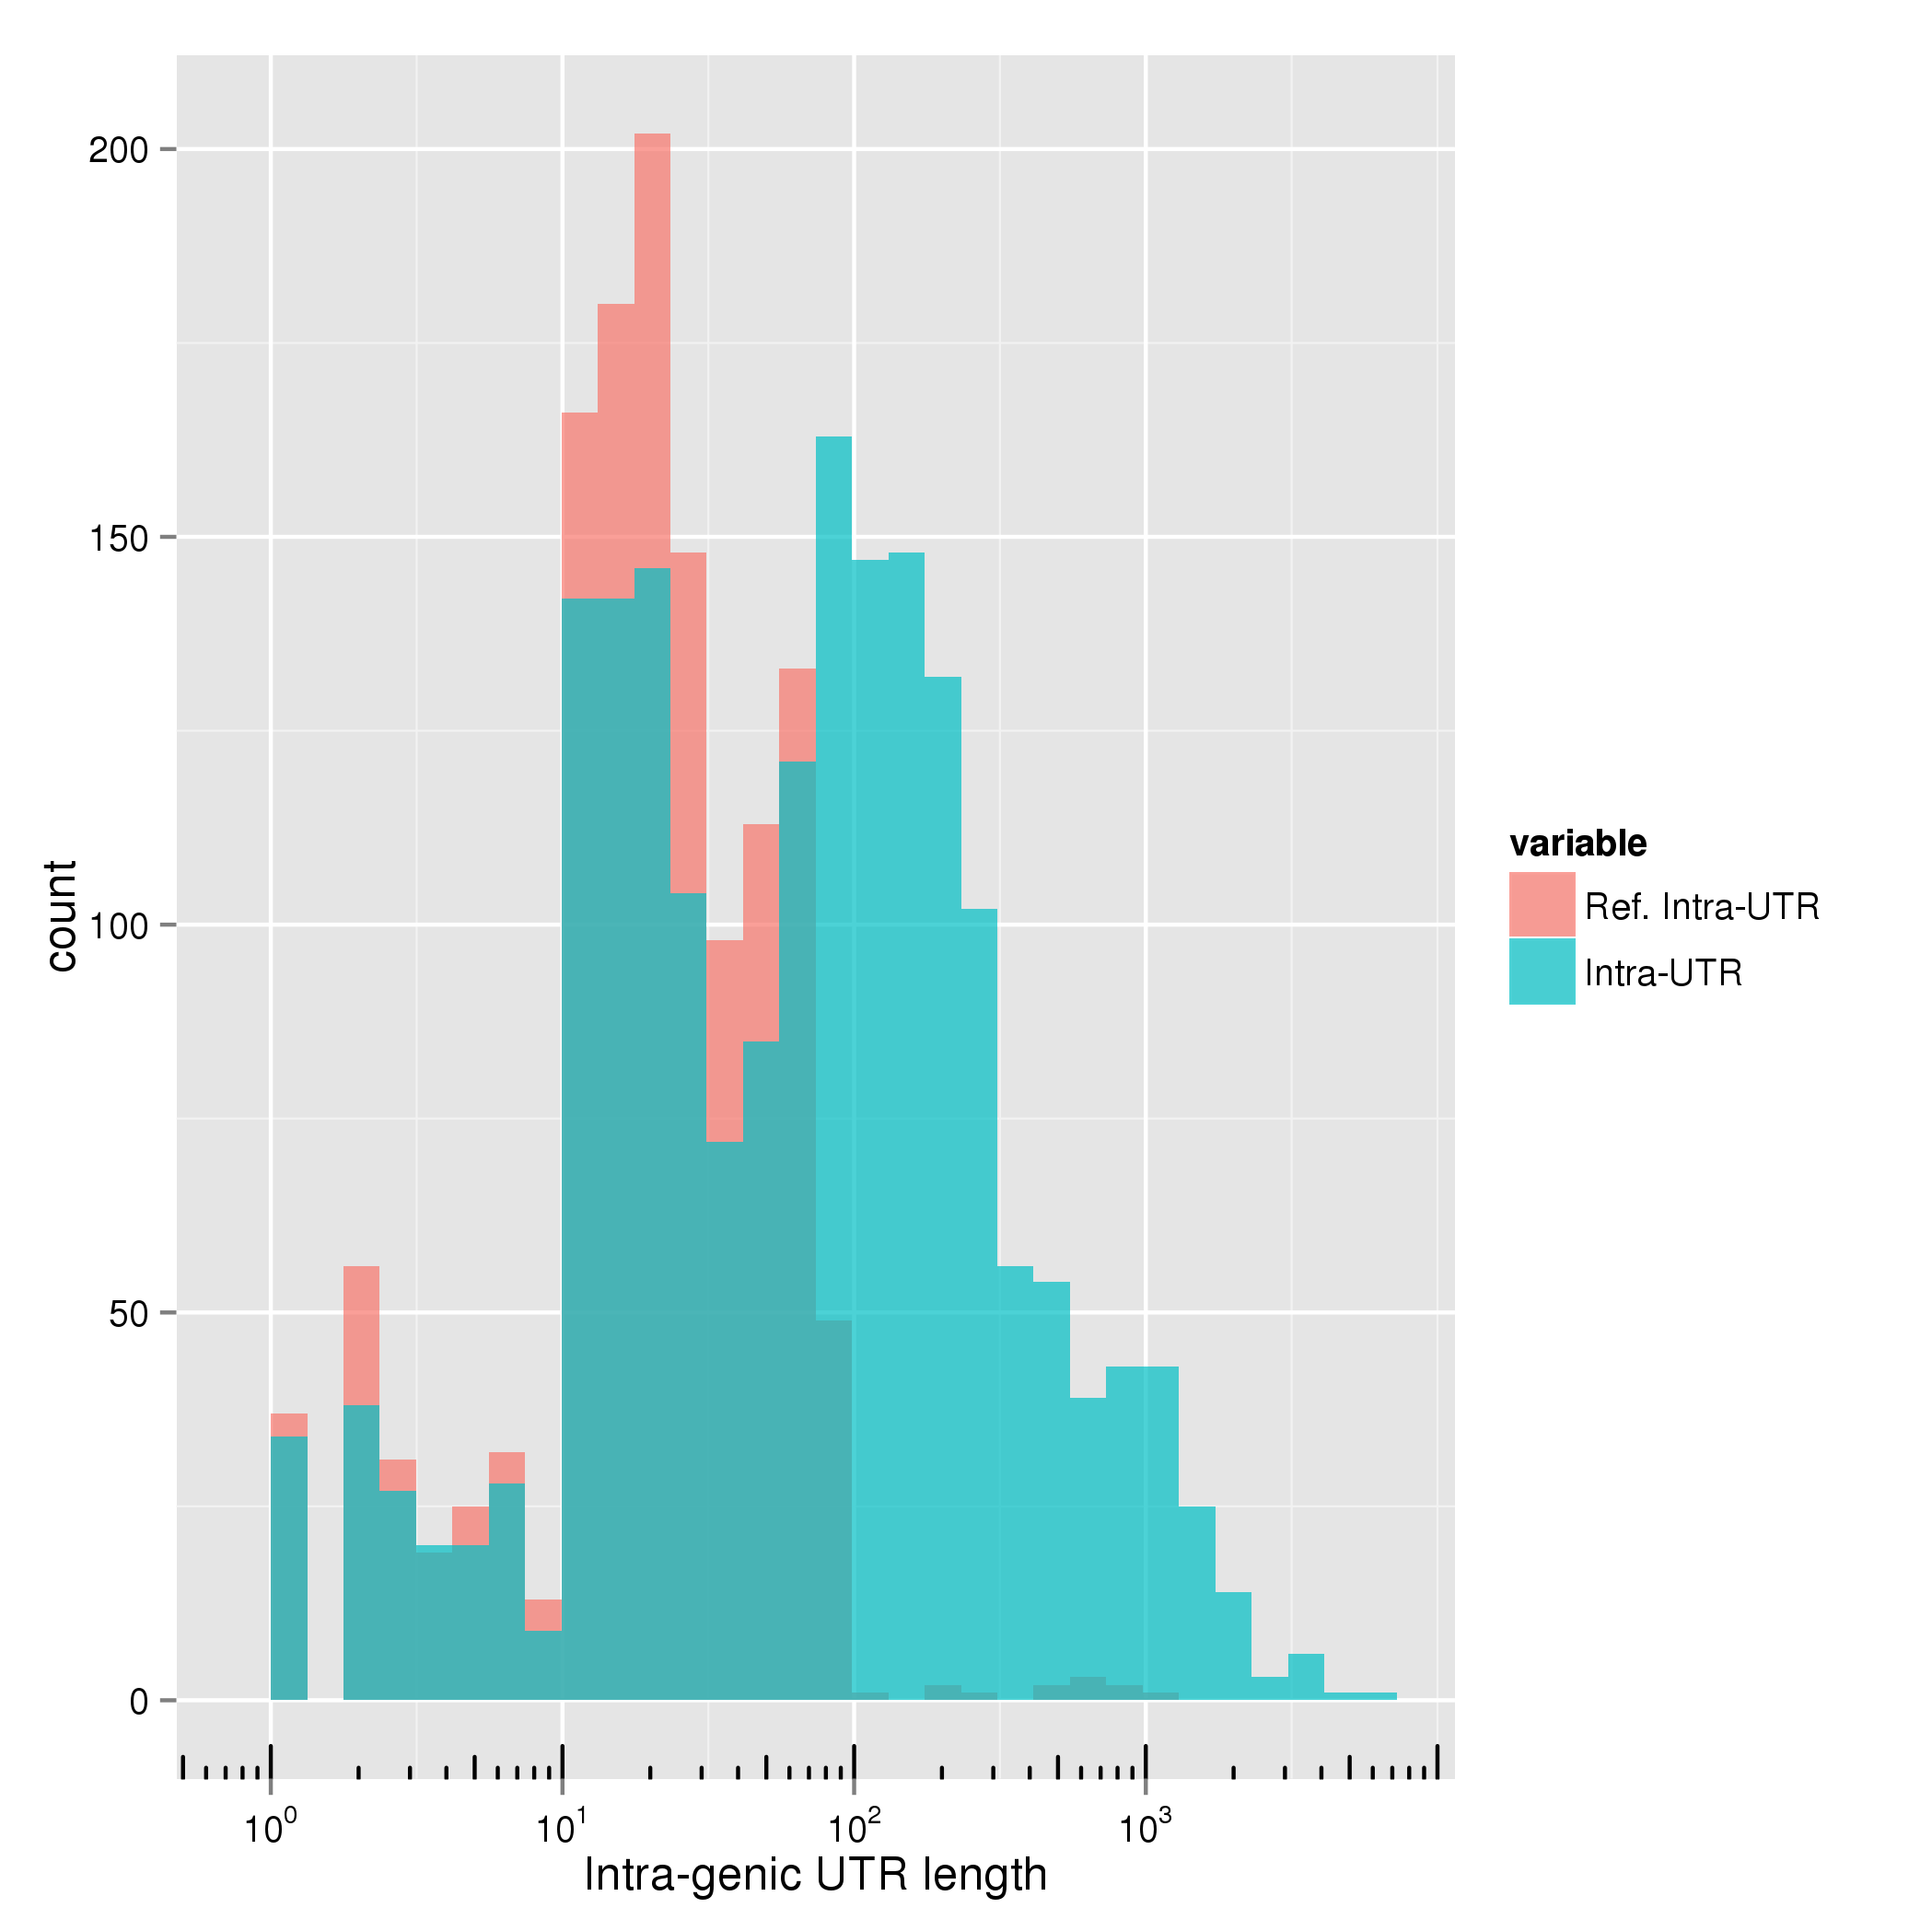
\includegraphics[width=\linewidth,height=3in]{images/Assembly/Summary/fintrautrlength_1.png}
\subcaption{Intra-operonic Untranslated Region}\label{fig:5.4b}}
\end{center}
\end{minipage}
\end{center}
\caption{Untranslated Regions}
The standard transcripts contain untranslated regions that suggest a level of misassembly, indicated by extended 5$\prime$ and 3$\prime$ UTRs (\subref{fig:5.4a}). The 3$\prime$ UTRs display a slightly bimodal pattern. Some of the extended UTRs may encode previously unannotated proteins or riboregulatory elements.
\end{figure}

A further illustration of misassembly can be seen in the distribution of untranslated region (UTR) lengths (\ref{fig:5.4a}). A number of the standard transcripts possess 5$\prime$ and 3$\prime$ UTRs that are several hundreds of basepairs in length, while most UTRs previously determined in \textit{C. acetobutylicum}\cite{63,64,69,74,76} and \textit{E. coli}\cite{87} are around 100bp. Some of these UTRs could contain riboswitches or unannotated proteins, although most likely not at the frequency shown by this histogram. Therefore, it is desirable to address these misassemblies through a curation process.

Encouraging results were obtained from examination of the uncurated assembly of the properly paired reads. This subset produced a large number of transcripts spanning 88\% of the bases of the genome and contained the majority of the reference protein annotations. The large number of assembled basepairs suggests good k-mer complexity in the data, indicating a truly diverse library, likely to contain rare and novel transcripts. Additionally, the large size of the initial assembly suggests that at least some signal is acquired for much of the genome, reducing the false negative rate and indicating high depth. Analysis of the novel transcripts by size and expression suggests that small RNAs and larger protein-encoding messages have been acquired in this dataset. As expected, false positive transcripts were assembled from technical artifacts such as background antisense signal and spurious transcription. These background signals are also apparent in the large UTR lengths of the standard transcripts. After seeing evidence of these novel transcripts, misassemblies, and background signals at a high level, it was desirable to closely examine and illustrate these examples. To investigate these issues, a customized genome browser was developed as a tool for curation to increase the precision and accuracy of the transcript coordinates.









